\title{Seislet-based morphological component analysis using exponential shrinkage}

\renewcommand{\thefootnote}{\fnsymbol{footnote}}

\author{Pengliang Yang\footnotemark[1], Sergey Fomel\footnotemark[2], Jinghuai Gao\footnotemark[1]}

\lefthead{P.L. Yang et al}
\righthead{Seislet-based MCA}

\address{
\footnotemark[1] Xi'an Jiaotong University\\
National Engineering Laboratory for Offshore Oil Exploration\\
Xi'an, China, 710049\\
\footnotemark[2] Bureau of Economic Geology,\\
John A. and Katherine G. Jackson School of Geosciences \\
The University of Texas at Austin \\
University Station, Box X \\
Austin, TX, USA, 78713-8924}


\setfigdir{Fig}

\maketitle

\begin{abstract}
Morphological component analysis (MCA) is a powerful tool used in image processing to separate different geometrical components (cartoons and textures, curves and points etc). MCA is based on the fact that many complex signals may not be sparsely represented using only one dictionary/transform, however can have sparse representation by combining several over-complete dictionaries/transforms. In this paper we propose seislet-based MCA for seismic data processing. MCA algorithm is reformulated as a shaping regularization paradigm. Successful seislet-based MCA depends on reliable slope estimation of seismic events, which is done by plane-wave destruction (PWD) filter. Due to the special importance of an effective shrinkage or thresholding function sparsity-promoting shaping optimization, we adopt an exponential shrinkage operator, which can flexibly  approximate many well-known existing thresholding functions. Numerical examples demonstrate the potential of seislet-based MCA in the application to trace interpolation, signal and noise separation as well as multiple removel.
\end{abstract}


\section{Introduction}

A wide range of applications have been carried out by solving a series of linear inverse problems, based on the fact that numerous varieties of signals can be sparsely represented with an appropriate dictionary, namely a certain kind of transform bases. Under the dictionary, the signals have fewer non-zeros of the representation coefficients. However, many complex signals are usually linear superposition of several elementary signals, and cannot be efficiently represented using only one dictionary. The concept of morphological diversity was therefore proposed by \cite{starck2004redundant,starck2005image} to combine several dictionaries for sparse representations of signals and images. Then, the signal is considered as a superposition of several morphological components. One has to chose a dictionary whose atoms match the shape of the geometrical structures to sparsify, while leading to a non-sparse (or at least not as sparse) representation of the other signal content. That is the essence of so-called morphological component analysis (MCA) \citep{starck2004redundant,starck2007undecimated,woiselle20113}.

Seislet transform and seislet frame are useful tools for seismic data compression and sparse representation \citep{fomel2010seislet}. Seislets are constructed by applying the wavelet lifting scheme \citep{sweldens1998lifting} along the spatial direction, taking advantage of the prediction and update steps to characterize local structure of the seismic events.
In seislet transform, the locally dominant event slopes are found by plane-wave destruction (PWD), which is constructed as finite difference stencils to characterize seismic images by a superposition of local plane waves \citep{claerbout1992earth}. By increasing the accuracy and dip bandwidth of PWD, \cite{fomel2002applications} demonstrated its competitive performance compared with prediction error filter (PEF) in the applications to fault detection, data interpolation, and noise attenuation. PWD keeps the number of adjustable parameters to a minimum, endows the estimated quantity with a clear physical meaning of the local plane-wave slope, and gets rid of the requirement of local windows in PEF. Recently, \cite{chen2013accelerated} accelerated the computation of PWD using an analytical estimator.


In this paper, we propose seislet-based MCA for seismic data processing. We reformulate MCA algorithm as a shaping regularization paradigm. Successful seislet-based MCA depends on reliable slope estimation of seismic events, which can be done by plane-wave destruction (PWD) filter. Due to the special importance of an effective shrinkage or thresholding function in sparsity-promoting shaping optimization, we propose an exponential shrinkage operator, which can flexibly  approximate many well-known existing thresholding functions. Numerical examples demonstrate the potential of seislet-based MCA in the application to trace interpolation, signal and noise separation as well as multiple removel.

\section{MCA with shaping regularization}

\subsection{Analysis-based iterative thresholding}

A general inverse problem combined with a priori constraint $R(x)$ can be written as an optimization problem
\begin{equation}\label{eq:sparsity3}
  \min_x \frac{1}{2}\|d_{obs}-K x\|_2^2+\lambda R(x),
\end{equation}
where $x$ is the model to be inverted, and $d_{obs}$ is the observations. To solve the problem with sparsity constraint $R(x)=\|x\|_1$, the iterative shrinkage-thresholding (IST) algorithm has been proposed  \citep{daubechies2004iterative}, which can be generally formulated as
\begin{equation}\label{eq:IST}
   x^{k+1}=T_{\lambda}(x^{k}+K^*(d_{obs}-Kx^{k})),
 \end{equation}
 where $k$ denotes the iteration number; $K^*$ indicates the adjoint of $K$. $T_{\lambda}(x)$ is an elementwise shrinkage operator with threshold $\lambda$:
 \begin{equation}
    T_{\lambda}(x)=(t_{\lambda}(x_1),t_{\lambda}(x_2),\ldots,t_{\lambda}(x_m))^T,
 \end{equation}
in which  the soft thresholding function \citep{donoho1995noising} is
 \begin{equation}
  t_{\lambda}(u)=\mathrm{Soft}_{\lambda}(u)=\left\{\begin{array}{ll}
                           u-\lambda\frac{u}{|u|}, & |u|> \lambda,\\
                           0, & |u|\leq \lambda.
                         \end{array}  \right.
	=u.*\max(1-\frac{\lambda}{|u|},0).
 \end{equation}

Allowing for the missing elements in the data, the observations are connected to the complete data via the relation
\begin{equation}
 d_{obs}=Md=M\Phi x=Kx, K=M\Phi.
 \end{equation}
where $M$ is a acquisition mask indicating the observed and missing values. Assume $\Phi$ is a tight frame such that $\Phi^*\Phi=\mathrm{Id}$, $x=\Phi^*\Phi x=\Phi^*d$. It leads to
\begin{equation}\label{eq:ist3}
  \begin{array}{ll}
    d^{k+1} & =\Phi x^{k+1} \\
      & =\Phi T_{\lambda}(\Phi^*d^{k}+(M\Phi)^*(d_{obs}-Md^{k})) \\
      & =\Phi T_{\lambda}(\Phi^*d^{k}+\Phi^*(M^*d_{obs}-M^*Md^{k})) \\
      & =\Phi T_{\lambda}(\Phi^*(d^{k}+(d_{obs}-Md^{k}))),
  \end{array}
\end{equation}
in which we use $M^*=M=(M)^2$ and $Md_{obs}=M^2d=Md$. Now we define a residual term as $r^{k}=d_{obs}-Md^{k}$, thus \eqref{eq:ist3} results in
\begin{equation}\label{eq:ist4}
  \left\{
  \begin{array}{l}
    r^{k}\leftarrow d_{obs}-Md^{k} \\
    d^{k+1}\leftarrow \Phi T_{\lambda}(\Phi^*(d^{k}+r^{k})),
  \end{array}
  \right.
\end{equation}
which is equivalent to solving
\begin{equation}\label{eq:ist5}
  \min\limits_{d}\frac{1}{2}\|d_{obs}-Md\|_2^2+\lambda R(\Phi^{*}d).
\end{equation}
Note that \eqref{eq:ist5} analyzes the target unknown $d$ directly, without resort to $x$ and $d=\Phi x$. \eqref{eq:ist3} is referred to as the analysis formula \citep{elad2007analysis}. This paper uses analysis formula because it directly addresses the problem in the data domain for the convenience of interpolation and signal separation.


\subsection{Understanding iterative shrinkage as shaping regularization}

Note that in each iteration soft thresholding is the only nonlinear operation which corresponds to the $\ell_1$ constraint for the model $x$, i.e., $R(x)=\|x\|_1$.
 Shaping regularization \citep{fomel2007shaping,fomel2008nonlinear} provides us a general and flexible framework so that we do not need to care too much about a specific constraint or penalty function $R(x)$ when a particular kind of shaping operator is used. The iterative shaping process can be expressed as
 \begin{equation}\label{eq:shaping1}
   x^{k+1}=S(x^{k}+B(d_{obs}-Fx^{k})),
 \end{equation}
where the shaping operator $S$ can be a smoothing operator \citep{fomel2007shaping}, or a more general operator even  a nonlinear sparsity-promoting shrinkage/thresholding operator \citep{fomel2008nonlinear}. The backward operator $B$ does not need to be the adjoint of the forward mapping $F$. It gives us more freedom to chose a form of $B$ to approximate the inverse of $F$ so that shaping regularization enjoys faster convergence rate in practice. In the language of shaping regularization, the updating rule in Eq. \eqref{eq:ist4} becomes
\begin{equation}\label{eq:shaping2}
  \left\{
  \begin{array}{l}
    r^{k}\leftarrow d_{obs}-Md^{k}, \\
    d^{k+1}\leftarrow \Phi S(\Phi^{*}(d^{k}+r^{k})),
  \end{array}
  \right.
\end{equation}
where the backward operator is chosen to be the inverse of the forward mapping.

 
\subsection{MCA using sparsity-promoting shaping}

MCA considers the complete data $d$ to be the superposition of several morphologically distinct components: $d=\sum_{i=1}^Nd_i$. For each component $d_i$, shaping-based MCA assumes there exists a transform $\Phi_i$ which can sparsely represent component $d_i$ by its coefficients $\alpha_i$ ($\alpha_i=\Phi_i^{*}d_i$ should be sparse), and can not do so for the others. Mathematically,
\begin{equation}\label{eq:mca_un}
  \min_{\{d_i\}}\sum_{i=1}^{N}R(\Phi^{*}d_i), s.t.\quad  d_{obs}=M\sum_{i=1}^{N}d_i.
\end{equation}
The above problem can be rewritten as
\begin{equation}\label{eq:mca1}
  \min_{\{d_i\}}\frac{1}{2}\left\|d_{obs}-M\sum_{i=1}^Nd_i\right\|_2^2+\lambda \sum_{i=1}^NR(\Phi^{*}d_i).
\end{equation}
We prefer to rewrite \eqref{eq:mca1} as
\begin{eqnarray}
  \min_{\{d_i\}}\frac{1}{2}\left\|\left(d_{obs}-M\sum_{j\neq i}d_j\right)-Md_i\right\|_2^2 \nonumber\\
   +\lambda R(\Phi_i^{*}d_i)+\lambda \sum_{j\neq i}R(\Phi_j^{*}d_j).
\end{eqnarray}
Thus, optimizing w.r.t. $d_i$ leads to the analysis IST shaping as \eqref{eq:shaping1}. At the \emph{k}th iteration, the shaping is performed alternatively for many components using block coordinate relaxation (BCR) technique \citep{bruce1998block}: for the \emph{i}th component $d_i^{k}$, $i=1,\ldots,N$: $\Phi\leftarrow \Phi_i$, $d^{k}\leftarrow d_i^{k}$, $d^{k+1}\leftarrow d_i^{k+1}$, $d_{obs}\leftarrow d_{obs}-M\sum_{j\neq i}d_j^{k}$, yields the residual term $r^{k}=d_{obs}-M\sum_{i=1}^N d_i^{k}$ and the updating rule
\begin{equation}\label{eq:mca2}
  \left\{
  \begin{array}{l}
    r^{k}\leftarrow d_{obs}-M\sum_{i=1}^N d_i^{k}  \\
    d_i^{k+1}\leftarrow \Phi_i S(\Phi_i^{*}(d_i^{k}+r^{k})).
  \end{array}
  \right.
\end{equation}
The final ouput of above algorithm are the morphological components $\hat{d}_i,i=1,\ldots,N$. The complete data can then be reconstructed via $\hat{d}=\sum_{i=1}^N \hat{d}_i$.
This is the so-called MCA-based inpainting algorithm \citep{Elad2005}.


\section{Seislet-based MCA sparsified with exponential shrinkage}

\subsection{Seislet transform and local slope estimation}

Seislet transform and seislet frame were proposed by \cite{fomel2010seislet} for seismic data compression and sparse representation. Seislets are constructed by applying the wavelet lifting scheme \citep{sweldens1998lifting} along the local slope direction. For each level of lifting decomposition, seismic data is split into even and odd parts ($\mathbf{e}$ and $\mathbf{o}$). Then the prediction and update step follows to obtain the detail difference/residual $\mathbf{d}$ and smooth information $\mathbf{s}$:
\begin{equation}
\mathbf{d}=\mathbf{e}-P[\mathbf{o}],\mathbf{s}=\mathbf{e}+U[\mathbf{d}].
\end{equation}
Recognizing that seismic data can be organized as collections of traces or records, \cite{fomel2010seislet} suggest prediction of one seismic trace or record from its neighbors and update of records on the next scale to follow structural features in seismic data. In the $Z$-transform notation the simplest Haar prediction filter can be written as
\begin{equation}
 P(Z)=Z,
\end{equation}
and the linear interpolation prediction filter is
\begin{equation}
 P(Z)=(Z+1/Z)/2.
\end{equation}
% To predict a particular frequency component $\omega_0$, we can use
% \begin{equation}
%  P(Z)=Z/Z_0, P(Z)=(Z/Z_0+Z_0/Z)/2,
% \end{equation}
% where $Z_0=e^{i\omega_0\Delta t}$.

Successful prediction and update plays a key role for local slope estimation. By modifying the biorthogonal wavelet construction, the prediction and update operators for a simple seislet transform are defined as
\begin{equation}
\begin{split}
 P[\mathbf{e}]_k=(S_k^{+}[\mathbf{e}_{k-1}] + S_{k}^{-} [\mathbf{e}_k]) /2,\\
 U[\mathbf{r}]_k=(S_k^{+}[\mathbf{r}_{k-1}] + S_{k}^{-} [\mathbf{r}_k]) /4,
\end{split}
\end{equation}
where $S_k^{+}$ and $S_k^{-}$ are operators that predict a trace from its left and right neighbors, corresponding to shifting seismic events in terms of their local slopes. The job of local slopes estimation can be done by PWD filters. Particularly, it is possible to obtain two or more dips with the help of PWD filters to capture different geometrical components of the seismic data. It is important to point out that besides PWD, there are many approaches to estimate dips of seismic data, i.e., local slant stack \citep{ottolini1983signal}, volumetric scan \citep{marfurt2006robust}. However, PWD provides us a computational efficient tool to obtain slope patterns and is therefore used in this work.


\subsection{Sparsifying MCA with exponential shrinkage shaping}

The IST algorithm used by MCA requires soft thresholding function to filter out the unwanted small values. Besides the soft thresholding \citep{donoho1995noising}, many other shrinkage function can also be applied to obtain possibly better sparseness. A popular choice is hard thresholding:
\begin{equation}
t_{\lambda}(u)=\mathrm{Hard}_{\lambda}(u)=u.*(|u|>\lambda?1:0).
\end{equation}
Another choice is Stein thresholding \citep{peyre2010advanced}:
\begin{equation}\label{eq:stein}
t_{\lambda}(u)=\mathrm{Stein}_{\lambda}(u)=u.*\max\left(1-(\frac{\lambda}{|u|})^{2},0\right).
\end{equation}
Stein thresholding does not suffer from the bias of soft thresholding, that is,
\begin{equation}
|\mathrm{Stein}_{\lambda}(u)-u| \rightarrow 0, |\mathrm{Soft}_{\lambda}(u)-u|\rightarrow \lambda,
\mathrm{if}\; u\rightarrow\infty.
\end{equation}
Recent advances in nonconvex optimization \citep{chartrand2012,chartrand2013generalized,chartrand2013nonconvex} show that the shrinkage operator in IST algorithm \eqref{eq:IST} can be generalized to a $p$-quasinorm ($0<p\leq1$) thresholding operator $T_{\lambda}$, in which
\begin{equation}\label{eq:pthresh}
t_{\lambda}(u)=\mathrm{pThresh}_{\lambda,p}(u)=u.*\max\left(1-(\frac{\lambda}{|u|})^{2-p},0\right).
\end{equation}
A special case is that of $p=1$, which corresponds to the soft thresholding operator exactly.



Most of these shrinkage functions interpolate between the hard and soft thresholders. It is tempting for us to design a more general shrinkage function to sparsify the transform domain coefficients in shaping regularized MCA. One possibility is  multiplying an exponential factor on the elements of original data:
\begin{equation}\label{eq:gen_op}
t_{\lambda}(u)=u.*\mathrm{exp}(-(\frac{\lambda}{|u|})^{2-p}).
\end{equation}
Based on Taylor series, this operator in \eqref{eq:gen_op} enjoys some nice properties:
\begin{itemize}
 \item For $|u|>>\lambda$, it is a good approximation of the p-thresholding operator in \eqref{eq:pthresh}, and does not suffer the bias when $p\neq 1$. It reduces to Stein thresholding operator for $p=0$ and soft thresholding for $p=1$. 
  \begin{equation}\label{eq:exp_sergey} 
  \begin{split}   
  t_{\lambda,0}(u)=u.*\mathrm{exp}(-(\frac{\lambda}{|u|})^{2})\approx u.*(1-(\frac{\lambda}{|u|})^{2}),\\
  t_{\lambda,1}(u)=u.*\mathrm{exp}(-(\frac{\lambda}{|u|}))\approx u.*(1-(\frac{\lambda}{|u|})).
  \end{split}
\end{equation}
 \item It is free of non-differentiable singularity at the thresholding point $\lambda$. The transition between the small values and the large values is smoothly stretched. Due to the expenential factor less than 1 ($\mathrm{exp}(-(\frac{\lambda}{|u|})^{2-p})<1$), this operator will slightly decrease the data amplitude, even for $|u|<\lambda$.
 \item Besides the threshold $\lambda$, we have another independent parameter $p$ which can be flexibly chosen to obtain best performance.
\end{itemize}
For the convenience of comparison, we plot these thresholding operators in Figure \ref{fig:thresh}. A critical point is that the exponential shrinkage function is devoted to diversifying the thresholding capability of seislet-based MCA instead of exhibiting better effect. It obtained competitive (sometimes better) sparsifying effects in our experiment compared with the existing thresholding operators.  By incorporating PWD dip estimation and exponential shrinkage shaping, we summarize the proposed seislet-based MCA algorithm in Algorithm \ref{algorithm:lpmca}. In fact, seislet transforms associated with different dips forms a combined seislet frame. Shrinkage operator plays an role of crosstalk removal in MCA algorithm, see more details in Appendex A.
%\begin{figure}
%\centering
%  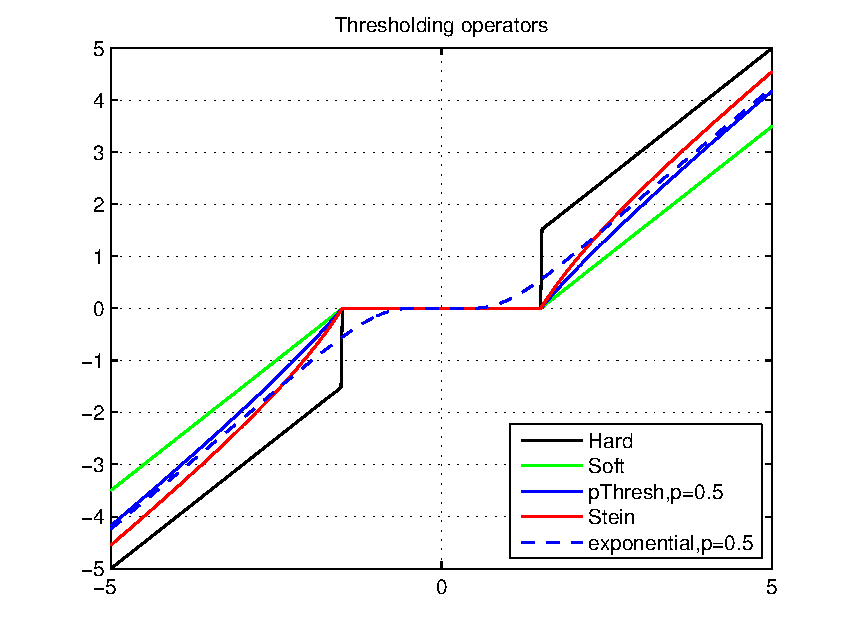
\includegraphics[width=\linewidth]{thresh}\\
%  \caption{A schematic plot of the shrinkage operators,$\lambda=1$}\label{fig:thresh}
%\end{figure}

  \plot{thresh}{width=0.7\linewidth}{A schematic plot of the shrinkage operators,$\lambda=1$}

\begin{algorithm}[htb]
    \caption{Seislet-based MCA algorithm}\label{algorithm:lpmca}
    \begin{algorithmic}[1]
    \renewcommand{\algorithmicrequire}{\textbf{Input:}}
    \REQUIRE Observed seismic image $d_{obs}$; sampling mask $M$; iteration number $niter$; shrinkage shaping parameter $p$, seislet transform $\Phi_i$  associated with the $i$th estimated slope.
    \renewcommand{\algorithmicensure}{\textbf{Output:}}
    \ENSURE Separated seismic component $d_i$.
    \STATE Initialize: $d_i^{(k)}\leftarrow 0$, $ i=1\ldots N$;
        \FOR {$k=1\ldots niter$}
            \STATE  $r^{(k)} \leftarrow d_{obs}-M\sum_{i=1}^N d_i^{(k)}$;
            \FOR{$i=1\ldots N$}
                \STATE  $x_i^{(k)}\leftarrow \Phi_i^*(d_i^{(k)}+r_i^{(k)})$;
                \STATE  Estimate shaping thresholder $\lambda$;
                \STATE  $d_i^{(k)}\leftarrow \Phi_i S(x_i^k) $;
            \ENDFOR
        \ENDFOR
    \end{algorithmic}
\end{algorithm}



\section{Numerical examples}

\subsection{Trace interpolation}

Interpolation of random missing traces is an important step in seismic data processing. Unlike most studies using only one transform, we consider the seismic data having two different components, which can be characterized by seislet transforms associated with two different slopes. PWD filter is utilized to estimate the two dip fields. As shown in Figure~\ref{fig:interp}, the complete data is decimated with a random eliminating rate 50\%. 10 iterations are performed to separate these components. The estimated dips (Figure~\ref{fig:dips}) by PWD are indicates that the separated two components exhibit different modes: component 2 has many conflicting seismic events (corresponding to positive and negative dips) while the events of component 1 are more consistent (most values of the dip are positive). The summation of the two components gives a reasonable interpolation result, see the last panel of Figure~\ref{fig:interp}.

%\begin{figure}
%\centering
%  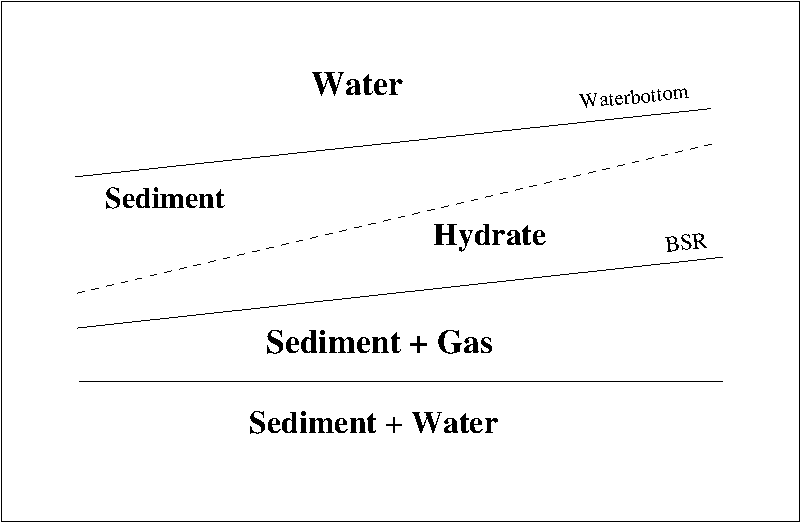
\includegraphics[width=\linewidth]{interp}\\
%  \caption{Simultaneous multi-component trace interpolation. From left to right: (a) Original complete seismic data, (b) data with 50\% random missing values, (c) component 1 and (d) component 2, (e) interpolated data.}
%\label{fig:interp}
%\end{figure}


\inputdir{interp}
  \plot{interp}{width=\linewidth}{Simultaneous multi-component trace interpolation. From left to right: Complete seismic data, data with 50\% random missing values, MCA interpolated component 1 and component 2, final interpolated data.}
  \plot{dips}{width=\linewidth}{PWD estimated dips: dip estimation for component 1 (Left) are positive-valued, while dip for component 2 includes negative and positive values.}



%
% \subsection{Separation of two shots}
%
% The second validation of seislet-based MCA is a test of shot separation. We do the numerical blending by simply reversing one shot in spatial axis and add the original shot and the reverse one together, shown in Figure~\ref{fig:blended}. Now, the data has no missing traces so that $M$ is an identity operator. Again, PWD filter is used for slope estimation. We feed the MCA routine with the estimated two dips (the top panels in Figure~\ref{fig:deblended}), leading to the final deblending result (the bottom panels of Figure~\ref{fig:deblended}).  It is important to point out that deblending is commonly performed by iterative denoising in an appropriate domain in which the crossing coherent seismic events from other sources becomes incoherent noise \citep{mahdad2011separation}.
%
%
% \begin{figure}
% \centering
%   \includegraphics[width=0.5\linewidth]{blended}\\
%   \caption{Numerically blended two shots} \label{fig:blended}
% \end{figure}
%
%
% \begin{figure}
% \centering
%   \includegraphics[width=0.8\linewidth]{deblended}\\
%   \caption{Top: (a--b) estimated two dips by PWD. Bottom: (c--d) deblended two shots.} \label{fig:deblended}
% \end{figure}




\subsection{Signal and noise separation}

A challenging problem in geophysical community is coherent noise elimination. To validate performance of seislet-based MCA for coherent noise attenuation, we conduct a benchmark synthetic test used by \cite{fomel2002applications}. As shown in Figure~\ref{fig:signalnoise}, the synthetic signal including consistent seismic events, is seriously contaminated by the synthetic dipping noise, which is so strong that we treat them as another signal component. From a geometrical point of view, PWD can estimate the slopes in a nice way. After 10 iterations of  seislet-based MCA computation, we obtain simultaneously separated signal and noise. As can be seen from the figure, the signal can be separated from the dipping noise favorably.

%\begin{figure}
%\centering
%  \includegraphics[width=0.8\linewidth]{signalnoise}\\
%  \caption{Simple example of dip-based signal and noise separation. From left to right: ideal signal, input data, estimated noise, estimated signal.}
%\label{fig:signalnoise}
%\end{figure}


\inputdir{sep1}
  \plot{signalnoise}{width=0.8\linewidth}{Simple example of dip-based signal and noise separation. From left to right: ideal signal, input data, estimated noise, estimated signal.}
  

\subsection{Multiple removal}

The last example is the separation of primaries and multiples for the field CMP data shown in Figure~\ref{fig:srme} \citep{fomel2006regularizing}. The multiples are predicted using surface-related multiple elimination (SRME). Even though SRME fails to predict the correct amplitudes, however, the resulting prediction helps PWD to extract the dominant slopes of the multiple events. 
Before applying the seislet-based MCA method, it is important to point out that the iterative reweighted least-squares (IRLS) method using the model precondition is another way for sparsity-enforced separation. The multiple removal is performed using three different methods: PWD-based IRLS method, seislet-based IRLS method, as well as the proposed seislet-based MCA method. For comparison, the separated primaries and multiples using different methods are plotted in Figures~\ref{fig:signal} and \ref{fig:nois}. Visually, the separated primaries by PWD-based IRLS method does not remove enough multiple contamination ( large amount of pigleg multiples still remains), while the seislet-based IRLS method and the seislet-based MCA method output similar primaries, which can also be seen clearly from the velocity scans of the primaries shown in Figure~\ref{fig:vsignal}. To further confirm our conclusion, we draw the velocity scans of predicted multiples in Figure~\ref{fig:vnois}. The panels of velocity scan in Figures~\ref{fig:vsignal} and \ref{fig:vnois} demonstrate that using MCA, the primaries correctly correspond to high speed part while the multiples are associated with slow speed part. Figure~\ref{fig:vnois} shows that seislet-based MCA outperforms seislet-based IRLS method in the deeper part of the velocity scan panel (see marked location A) due to the best match of the corresponding semblance scan of the original data. Note that the seislet-based MCA algorithm only uses 15 iterations to obtain the best separation effect, while the number of iterations for PWD-IRLS method and seislet-IRLS method are 10000 and 1000, respectively. Therefore, seislet-based MCA is very efficient to demultiple.


% \begin{figure}
% \centering
%   \includegraphics[width=0.8\linewidth]{srme}\\
%   \caption{The field CMP data (left) and SRME predicted multiples (right).The field CMP data (left) and SRME predicted multiples (right). The amplitudes of SRME prediction needs to be corrected.}
% \label{fig:srme}
% \end{figure}
% 
% \begin{figure}
% \centering
%   \includegraphics[width=0.8\linewidth]{signal}\\
%   \caption{Separated primaries using PWD (10000 iterations), weighted seislet optimization (1000 iterations) and seislet-based MCA (15 iterations).}
% \label{fig:signal}
% \end{figure}
% 
% \begin{figure}
% \centering
%   \includegraphics[width=0.8\linewidth]{nois}\\
%   \caption{Separated multiples using PWD (10000 iterations), weighted seislet optimization (1000 iterations) and seislet-based MCA (15 iterations).}
% \label{fig:nois}
% \end{figure}
% 
% \begin{figure}
% \centering
%   \includegraphics[width=0.8\linewidth]{vsignal}\\
%   \caption{Velocity scan for primaries obtained by PWD, weighted seislet optimization and seislet-based MCA (from left to right). The velocity scan of original data is shown in the last panel for comparison.}
% \label{fig:vsignal}
% \end{figure}
% 
% \begin{figure}
% \centering
%   \includegraphics[width=0.8\linewidth]{vnois}\\
%   \caption{Velocity scan for multiples obtained by PWD, weighted seislet optimization seislet-based MCA (from left to right). The velocity scan of original data is shown in the last panel for comparison. In the deeper part (location A) the velocity scan panel of separated multiples using seislet-MCA can best conform to the corresponding semblance scan of the original data.}
% \label{fig:vnois}
% \end{figure}


\inputdir{sep2}
  \plot{srme}{width=0.7\linewidth}{The field CMP data (left) and SRME predicted multiples (right). The amplitudes of SRME prediction needs to be corrected.}
  
  \plot{signal}{width=0.8\linewidth}{Separated primaries using PWD-IRLS (10000 iterations), seislet-IRLS (1000 iterations) and seislet-based MCA (15 iterations).}
  
  \plot{nois}{width=0.8\linewidth}{Separated multiples using PWD-IRLS (10000 iterations), seislet-IRLS (1000 iterations) and seislet-based MCA (15 iterations).}

  \plot{vsignal}{width=\linewidth}{Velocity scan for primaries obtained by PWD-IRLS, seislet-IRLS and seislet-based MCA (first three panels, from left to right). The velocity scan of original data is shown in the last panel for comparison.}

  \plot{vnois}{width=\linewidth}{Velocity scan for multiples obtained by PWD-IRLS, seislet-IRLS and seislet-based MCA (first three panels, from left to right). The velocity scan of original data is shown in the last panel for comparison. The deeper part (location A) in the velocity scan panel of separated multiples using seislet-MCA can best match the semblance scan of the original data, compared to the others.}
  
\section{Conclusion and discussion}

We have developed a seislet-based MCA method for seismic data processing. PWD filter can be utilized to estimate the slopes of seismic data. An exponential shrinkage function is introduced to diversify the capability of sparsity-promoting shaping operator. The proposed seislet-based MCA using shaping regularization is promosing in the application to seismic trace interpolation, signal and noise separation, as well as multiple removal. 

The sparsity-promoting shaping regularization plays an extremely important role in successful seislet-based MCA separation. The parameters needs to be set according to empirical experiments.  Our experience show that there is little difference to choose different thresholding functions for the same parameters. However, the special importance of the proposed exponential shrinkage operator is that it is free of non-differential sigularity and unifies many existing shrinkage operators.


\section*{Acknowledgments}

The work of the first author is supported by China Scholarship Council during his visit to Bureau of Economic Geology, University of Texas at Austin. We would like to thank Wenchao Chen and Jianwei Ma for valuable discussions. The numerical examples are reproducible with  Madagascar software package \citep{m8r}.

\append{Seislet frame in MCA algorithm}
\label{app:seisletframe}

The complete data $d$ is regarded to be superposition of several different geometrical components, and each component can be sparely represented using a seislet dictionary $\Phi_i$, i.e.,
\begin{equation}
\begin{array}{ll}
  d&=\sum_{i=1}^N d_i=\sum_{i=1}^N \Phi_i \alpha_i\\
  &=[\Phi_1,\Phi_2,\cdots,\Phi_N]\left[\begin{array}{l}
                                        \alpha_1\\
                                        \alpha_2\\
                                        \vdots\\
                                        \alpha_N
                                       \end{array}
\right]\\
\end{array}
\end{equation}
where $F=[\Phi_1,\Phi_2,\cdots,\Phi_N]$ is a combined seislet dictionary (i.e. seislet frame up to a constant), and the backward operator is chosen to be
\begin{equation}
 B=\left[\begin{array}{l}
                \Phi_1^{*}\\
		\Phi_2^{*}\\
                \vdots\\
                \Phi_N^{*}
   \end{array} \right]
\end{equation}
in the sense that
\begin{equation}
 FB=\sum_{i=1}^N\Phi_i\Phi_i^{*}=N \mathrm{Id}.
\end{equation}
Recall that we are using BCR technique to sparsify one component while keeping all others fixed. At the $k+1$-th iteration applying the backward operator on the $i$-th component leads to
\begin{equation}
\tilde{\alpha}_i^{k+1}=\alpha_i^k+\sum_{i=1}^N\Phi_i^{*} r^k=\alpha_i^k+r_i^j+\sum_{j\neq i}\Phi_i^{*} r_j^k
\end{equation}
where the terms $\sum_{j\neq i}\Phi_i^{*}r_j^k$ are the crosstalk between the $i$-th component and the others. An intuitive approach to filter out the undesired crosstalk is shrinkage/thresholding. The proposed exponential shrinkage provides us a flexible tool to approximate the performance of existing shrinkage/thresholding functions.

\bibliographystyle{seg}  % style file is seg.bst
\bibliography{mcaseislet}

